\chapter{Machine Thermique} % (fold)
\label{chap:Machine Thermique}

\section{Transformation cyclique} % (fold)
\label{sec:Transformation cyclique}

\subsection{Moteurs et récpteurs} % (fold)
\label{sub:Moteurs et récpteurs}

% subsection Moteurs et récpteurs (end)

\subsection{Répresentation en diagramme} % (fold)
\label{sub:Répresentation en diagramme}

\subsubsection{Diagramme de Clapeyron} % (fold)
\label{sec:Diagramme de Clapeyron}

% subsubsection Diagramme de Clapeyron (end)
% subsection Répresentation en diagramme (end)

\subsection{Bilans sur un cycle} % (fold)
\label{sub:Bilans sur un cycle}

Au cours d'un cycle, toutes les grandeurs d'état reste inchangée.

\begin{itemize}

    \item Bilan d'énergie interne : 
      \begin{equation}
        [U] _i ^{f} = 0 \implies W + Q = 0
      \end{equation}

    \item Bilan d'entropie : 
      \begin{equation}
        [S] _ i ^{f} = 0 \implies S _{cr} + S _{ech} = 0
      \end{equation}
\end{itemize}
% subsection Bilans sur un cycle (end)

\subsection{Machines monotherme : impossible} % (fold)
\label{sub:Machines monotherme : impossible}

\begin{equation}
  Q = T_0 S _{ech} = - T_0 S _{cr} \le _{rev} 0 \implies W \ge _{rev} 0
\end{equation}

\textbf{Conclusion} : Il est impossible de réaliser un moteur avec un cycle monotherme.
% subsection Machines monotherme : impossible (end)

\subsection{Machines multithermes} % (fold)
\label{sub:Machines multithermes}

\subsubsection{Inégalité de Clausius} % (fold)
\label{sec:Inégalité de Clausius}

\begin{equation}
  \sum_{i}^{} \frac{Q_i}{T_i}  \le _{rev} 0
\end{equation}
% subsubsection Inégalité de Clausius (end)
% subsection Machines multithermes (end)
% section Transformation cyclique (end)

\newpage
\section{Machines dithermes} % (fold)
\label{sec:Machines dithermes}

\begin{tcolorbox}
  \textbf{Notations} : Pendant un cycle, le système $\Sigma$ \underline{reçoit} la chaleur $Q_C$ de la part de la source chaude de température $T_C$, de même façon \underline{reçoit} $Q_F$ de celle de $T_F$.
\end{tcolorbox}
\subsection{Diagramme de Raveau} % (fold)
\label{sub:Diagramme de Raveau}

\begin{figure}[H] %h:当前位置, t:顶部, b:底部, p:浮动页
  \centering
  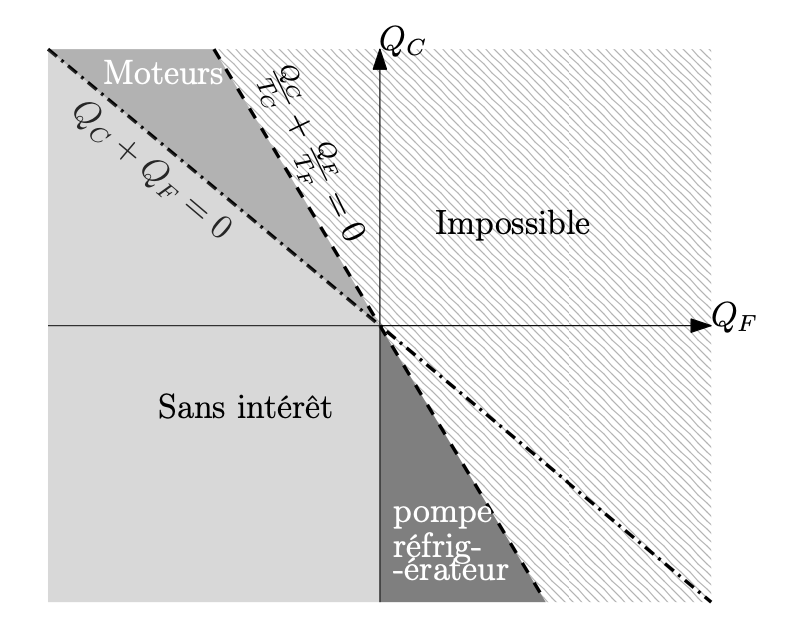
\includegraphics[width=0.6\textwidth]{./assets/Diagramme de Raveau.png}
  \caption{Diagramme de Raveau}
  \label{fig:Diagramme de Raveau}
\end{figure}

Explication : 
\begin{itemize}

    \item Droites :
      \begin{equation}
        \frac{Q_C}{T_C}  + \frac{Q_F}{T_F}  < 0 \implies Q_C < - \frac{T_C}{ T_F}  Q_F \text{ avec } \frac{T_C}{T_F}  > 1
      \end{equation}

    \item La domaine des \underline{moteurs} : 
      \begin{equation}
        Q_C > 0, \; Q_F < 0 ,\; W = - (Q_C + Q_F) < 0
      \end{equation}

    \item La domaine des \underline{récepteurs} : 
      \begin{equation}
        Q_C < 0, \; Q_F > 0, \; W = - (Q_C + Q_F) > 0
      \end{equation} 

\end{itemize}

% subsection Diagramme de Raveau (end)
% section Machines dithermes (end)

\subsection{Efficacité thermodynamique} % (fold)
\label{sub:Efficacité thermodynamique}

\subsubsection{Définition} % (fold)
\label{sec:Définition}

\begin{itemize}

    \item \textbf{Efficacité thermodynamique} : 
      \begin{equation}
        e = \frac{\text{ce que l'on veut}}{\text{ce que l'on paye}} 
      \end{equation} 
    \item \textbf{Rendement} : 
      \begin{equation}
        \eta = \frac{e _{\text{réelle}}}{e _{\text{théorique}}} 
      \end{equation}

\end{itemize}

\subsubsection{Moteur : efficacité de Carnot} % (fold)
\label{sec:Moteur : efficacité de Carnot}

L'efficacité du moteur est limitée par : 
\begin{equation}
  e  = \frac{-W}{Q_C} \le _{rev} e_c = 1 - \frac{T_F}{T_C} 
\end{equation}
% subsubsection Moteur : efficacité de Carnot (end)
% subsubsection Définition (end)
% subsection Efficacité thermodynamique (end)

\subsubsection{Machine frigorifique : efficacité frigorifique de Carnot} % (fold)
\label{sec:Machine frigorifique}

L'efficacité : 
\begin{equation}
  e  = \frac{Q_F}{W}  \le _{rev} e _{fr,c} =  \frac{T_F}{T_C- T_F} 
\end{equation}

\begin{myproof}{}{}
\begin{equation}
  \frac{Q_F}{W}  = \frac{Q_F}{-(Q_F+Q_C)}  = \frac{1}{ - 1 + \frac{Q_C}{Q_F} }  \le _{rev} - \frac{1}{ 1- \frac{T_C}{T_F} } 
\end{equation}
\end{myproof}


\begin{tcolorbox}
    \textbf{Note} : Il faut comprendre que $Q_F$ représente : on \underline{tire le chaleur de la source froide} (à l'intérieur) et de donner de la chaleur à la source chaude. $Q_F$ est considéré chaleur \underline{reçu} donc il est positif.
\end{tcolorbox}
% subsubsection Machine frigorifique (end)


\subsubsection{Pompe à chaleur} % (fold)
\label{sec:Pompe à chaleur}

\begin{equation}
  e = -\frac{Q_C}{W}  \le _{rev} e _{th,c} = \frac{T_C}{T_C - T_F}  
\end{equation}

\begin{tcolorbox}
    \textbf{Note} : On souhaite de \underline{donner de la chaleur à la source chaude} (intérieur, en hiver) en la prélevant à la source froide.
\end{tcolorbox}
% subsubsection Pompe à chaleur (end)

\subsection{Cycle de Carnot} % (fold)
\label{sub:Cycle de Carnot}

\subsubsection{Condition de réversibilité} % (fold)
\label{sec:Condition de réversibilité}

Dans un cycle ditherme \underline{réversible} (isentropique) : 
\begin{itemize}

    \item Quand il échange de chaleur avec un thermostat, la température du système doit rester inchangé. 

    \item La reste du cycle doit être isentropique = adiabatique réversible.

\end{itemize}

Donc, le cycle de Carnot est impossible à réaliser en pratique.

\subsubsection{Représentation pour un gaz parfait} % (fold)
\label{sec:Représentation pour un gaz parfait}

La courbe consiste à deux parties : 
\begin{itemize}

    \item partie isotherme : $PV = nRT_F$ et $PV = nRT_C$ 
    \item partie isentropique : Loi de Laplace donne $PV ^{\gamma} = C _{te}$

\end{itemize}

\begin{figure}[H] %h:当前位置, t:顶部, b:底部, p:浮动页
  \centering
  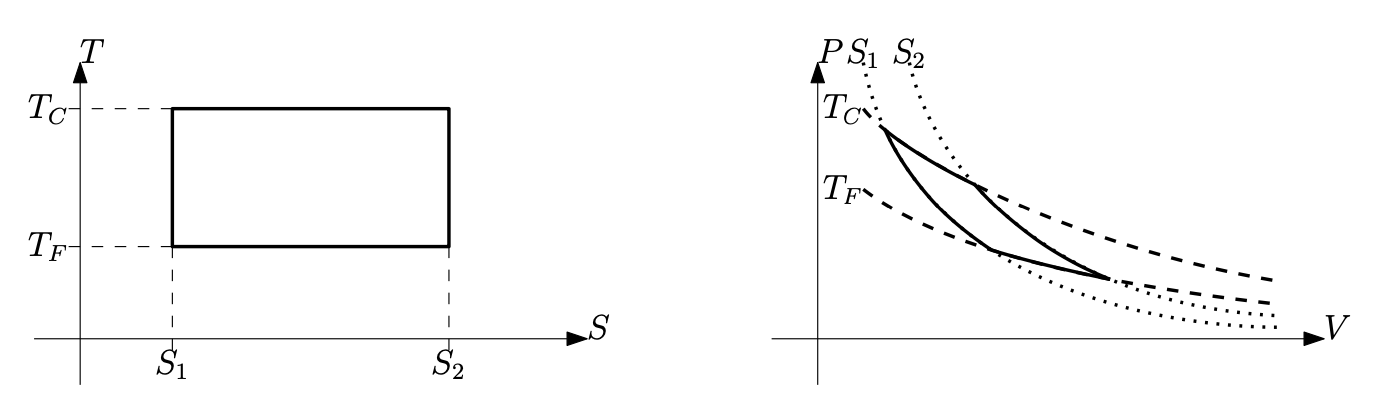
\includegraphics[width=0.8\textwidth]{./assets/Cycle de Carnot (GP).png}
  \caption{Cycle de Carnot (GP)}
  \label{fig:Cycle de Carnot (GP).png}
\end{figure}


% subsubsection Représentation pour un gaz parfait (end)
% subsubsection Condition de réversibilité (end)
% subsection CYcle de Carnot (end)

\subsection{Exemple : Cycle de Beau de Rochas} % (fold)
\label{sub:Exemple : Cycle de Beau de Rochas}

\begin{figure}[H] %h:当前位置, t:顶部, b:底部, p:浮动页
  \centering
  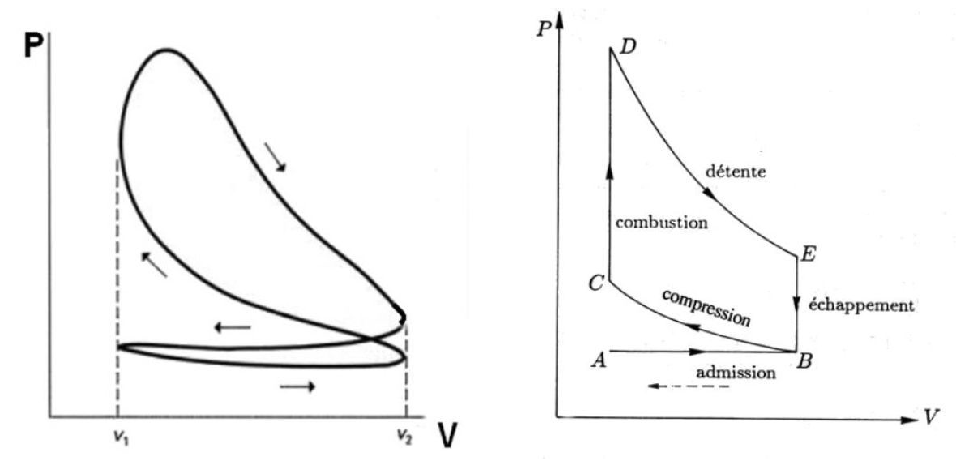
\includegraphics[width=0.8\textwidth]{./assets/Cycle de Beau de Rochas 1.png}
  \caption{Cycle de Beau de Rochas}
\end{figure}

\begin{figure}[H] %h:当前位置, t:顶部, b:底部, p:浮动页
  \centering
  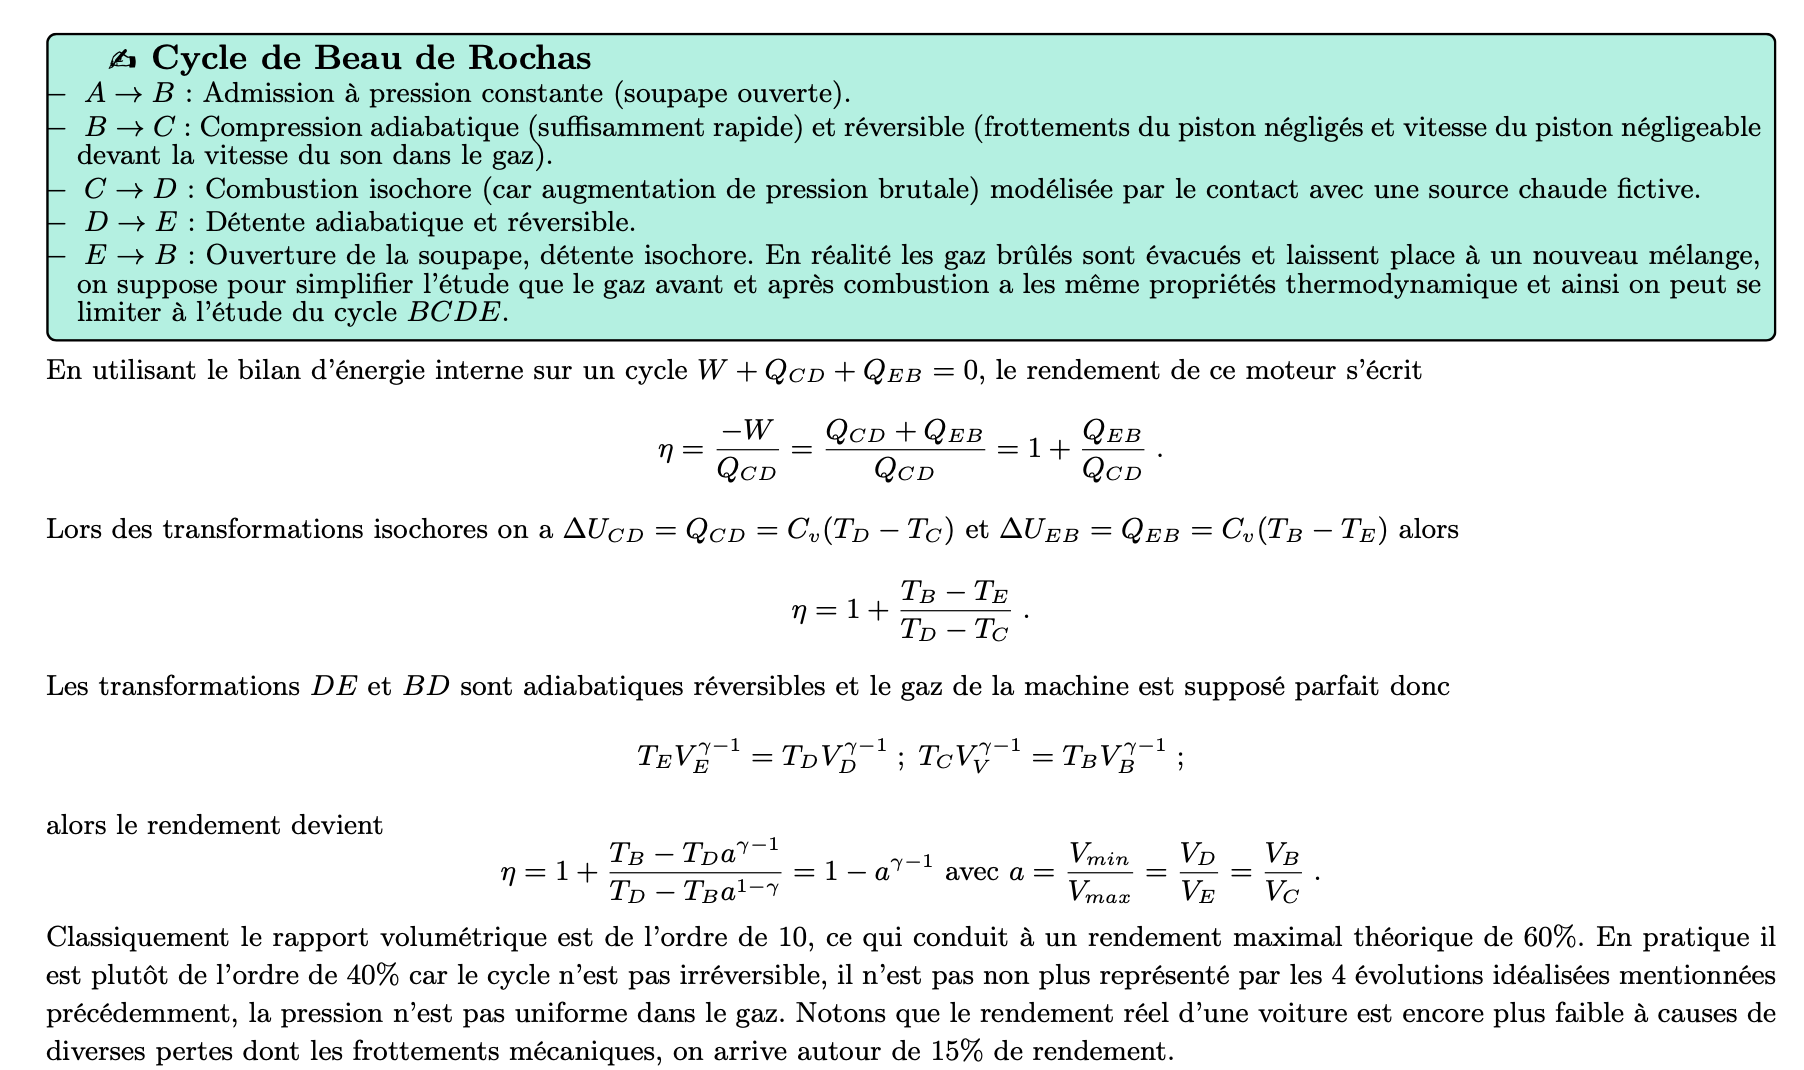
\includegraphics[width=1\textwidth]{./assets/Cycle de Beau de Rochas 2.png}
\end{figure}




% subsection Exemple : Cycle de Beau de Rochas (end)
 (end)
\subsection{Exemple : Machines frigorifiques} % (fold)
\label{sub:Exemple : Machines frigorifiques}

\begin{figure}[H] %h:当前位置, t:顶部, b:底部, p:浮动页
  \centering
  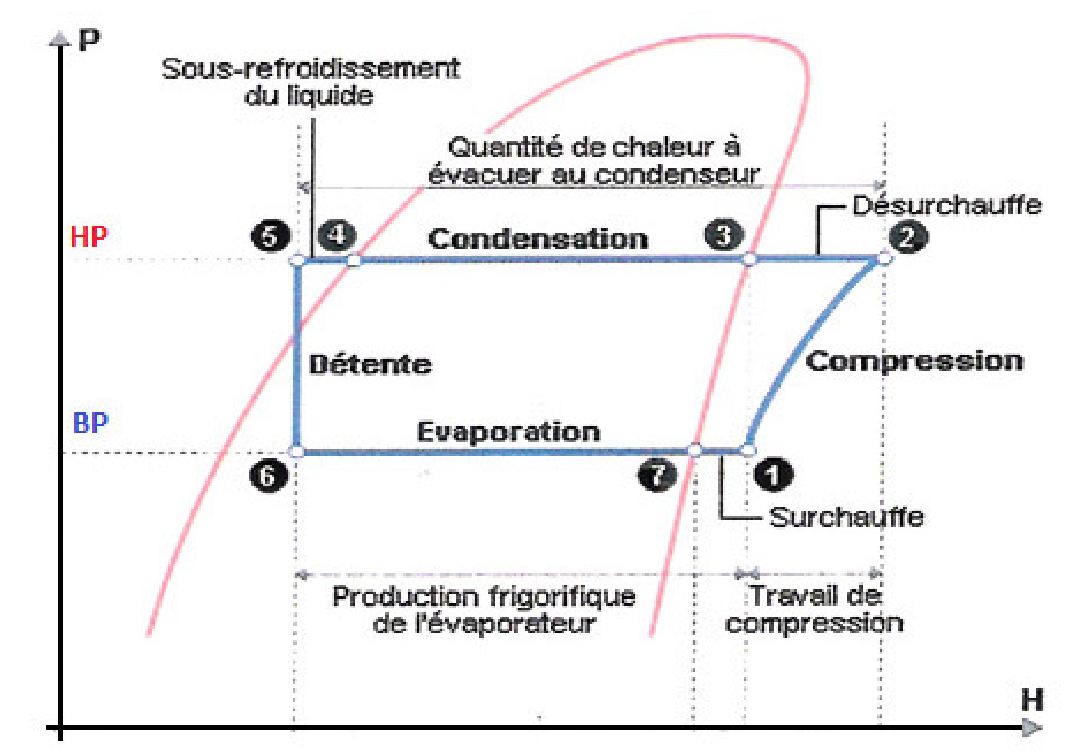
\includegraphics[width=0.8\textwidth]{./assets/Machines frigorifiques 1.png}
  \caption{Machines frigorifiques}
\end{figure}

\begin{figure}[H] %h:当前位置, t:顶部, b:底部, p:浮动页
  \centering
  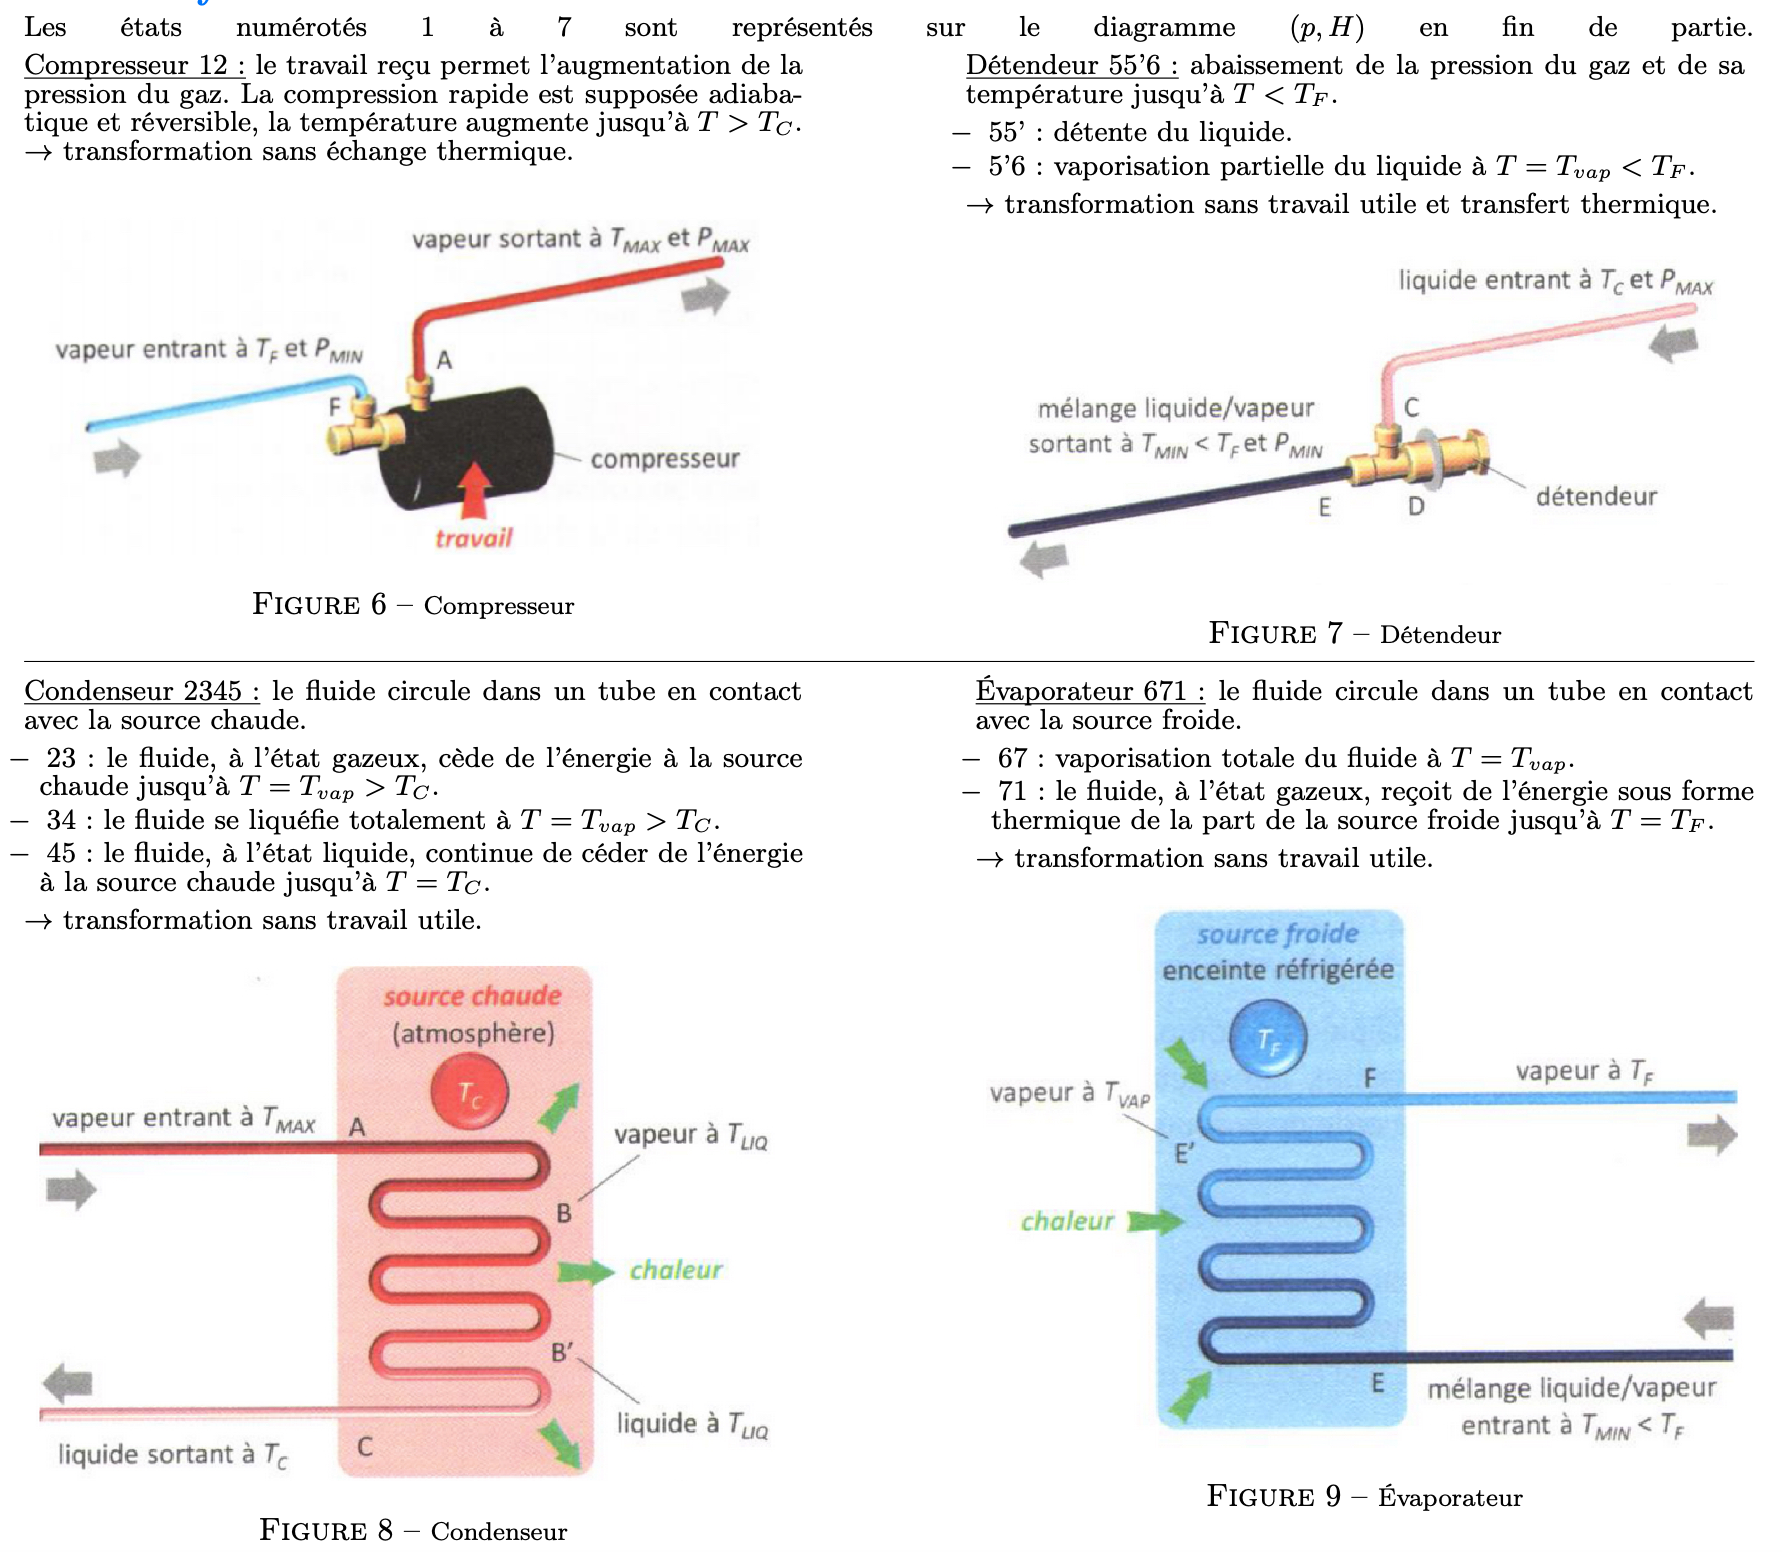
\includegraphics[width=\textwidth]{./assets/Machines frigorifiques 2.png}
\end{figure}



% subsection Exemple : Machines frigorifiques (end)
% section  (end)

\newpage 
\section{Dispositifs avec fluide en écoulement} % (fold)
\label{sec:Dispositifs avec fluide en écoulement}

\subsection{Généralités} % (fold)
\label{sub:Généralités}

\subsubsection{Bilan de masse} % (fold)
\label{sec:Bilan de masse}

% subsubsection Bilan de masse (end)
% subsection Généralités (end)

\begin{figure}[H] %h:当前位置, t:顶部, b:底部, p:浮动页
  \centering
  \includegraphics[width=0.8\textwidth]{./assets/Système d'étude.png}
  \caption{Système d'étude}
  \label{fig:Système d'étude}
\end{figure}




Considérons le système fermé $\Omega$ constitué de la matière qui, à l'instant $t$ se trouve entre $I$ et $O$. Une courte durée $\mathrm{d}t$ plus tard, $\Omega$ se \underline{retrouve} entre $I'$ et $O'$. 

Notons $M ^{*}(t)$ la masse de $\Omega$, à l'instant $t$. 
\begin{itemize}

    \item Système fermé : $M ^{*}( t+ \mathrm{d} t) = M ^{*}(t)$ 
    \item $M ^{*}(t + \mathrm{d} t) = M _{I'O} + M _{OO'}$, $M ^{*}(t) = M _{II'}+ M _{I'O}$

\end{itemize}

En régime permanent, donc $M _{OO' }- M _{II' }= 0$, avec la définition de \textbf{débits massiques} : 
\begin{equation}
  M _{OO'} = D_e \mathrm{d} t, \; M _{II'} = D_s \mathrm{d} t \implies D_e = D_s = D
\end{equation}
% subsection Bilan de masse (end)

\subsubsection{Bilan d'un grandeur extensive quelconque} % (fold)
\label{sec:Bilan d'un grandeur extensive quelconque}

\begin{equation}
  \frac{\mathrm{d}X ^{*}}{ \mathrm{d}t}  = D [x] _{e} ^{s}
\end{equation}
% subsubsection Bilan d'un grandeur extensive quelconque (end)

\subsection{Échange énergétique} % (fold)
\label{sub:Échange énergétique}

Le premier principe : 
\begin{equation}
  \left[ h + \frac{v ^{2}}{2}  \right] _{e} ^{s} = w _{mec} + q
\end{equation}

avec $w _{mec}$ est le travail reçu pour chaque unité de fluide
% subsection Échange énergétique (end)
% section Dispositifs avec fluide en écoulement (end)
% chapter Machine Thermique (end)
